\documentclass[pdf]{beamer}

\usepackage{graphicx}

\mode<presentation>{}

\title{A good programming language is a \textit{Functional} one}
\author{Artin Ghasivand}

\begin{document}

\begin{frame}
  \titlepage
\end{frame}

\section{Models of Computation}
\label{sec:models-of-computation}

\section{History of Programming Languages}
\label{sec:history}

\section{Functional Programming}
\label{sec:fp}

\begin{frame}{Languages}
  \begin{itemize}
  \item Haskell
  \item Emacs Lisp
  \item Racket
  \item Common Lisp
  \item Scheme
  \item Clojure
  \item Erlang
  \item Gleam
  \item SML
  \item Elixir
  \item OCaml
  \item F\#
  \item Miranda
  \item Hope
  \item Elm
  \item Idris
  \item Lean4
  \item Scala
  \end{itemize}
\end{frame}

\begin{frame}{Lisp}
  Short for \textit{List Processing}, Lisp is a family of \textit{Meta} programming languages based on the Untyped Lambda-Calculus first specified by John McCarthy.

  Inventions of Lisp:
  \begin{itemize}
  \item Garbage collection
  \item Read-Eval-Print Loop, n.e. REPL
  \item Dynamic Typing
  \item Conditionals
  \item Higher-Order functions
  \item Recursion
  \end{itemize}
\end{frame}

\begin{frame}{Haskell}
  NOTE: Some of these are probably not appropriate for the talk
  \begin{itemize}
  \item Referential Transparency
  \item Purity
  \item Laziness
  \item Type Classes (ad-hoc polymorphism)
  \item Type Inference
  \item Impredicative Instantiation
  \item Generalized Algebraic Datatypes
  \item Existential Types
  \item Type Families
  \item Guards
  \item Type Abstractions
  \item Higher-Rank Types
  \item Kind Polymorphism
  \item Dependent Kinds
  \end{itemize}

\end{frame}

\begin{frame}{Data Constructors and Patterns}
  The same tools that let me put some \textit{data} together allows us to take it apart.
  TODO Talk about data constructors and pattern matching
\end{frame}

\begin{frame}
  Lazy Evaluation, is an evaluation model where things get evaluated only when they \textit{need} to.

  Benefits of Laziness: (TODO Find more stuff)
  \begin{itemize}
  \item Infinite data structures
  \item Defining control-flow as functions instead of primitives or macros
  \item Lazy programs tend to terminate more than strict ones (TODO Double check)
  \item \textit{Forces} purity (TODO This may be unrelated and maybe you should just remove it)
  \end{itemize}
\end{frame}

\section{Types}
\label{sec:types}

\begin{frame}[fragile]{Type Inference}
\begin{verbatim}
and True x  = x
and False _ = False
\end{verbatim}

  Haskell is smart enough to \textit{infer} the type of \verb|and|, \verb|Bool -> Bool -> Bool|, by itself, and if you give it the wrong argument, it will tell you exactly what you did wrong!

  e.g. \verb|test = and True 'c'| will result in the following error message:
  \begin{figure}[H]
    \centering
    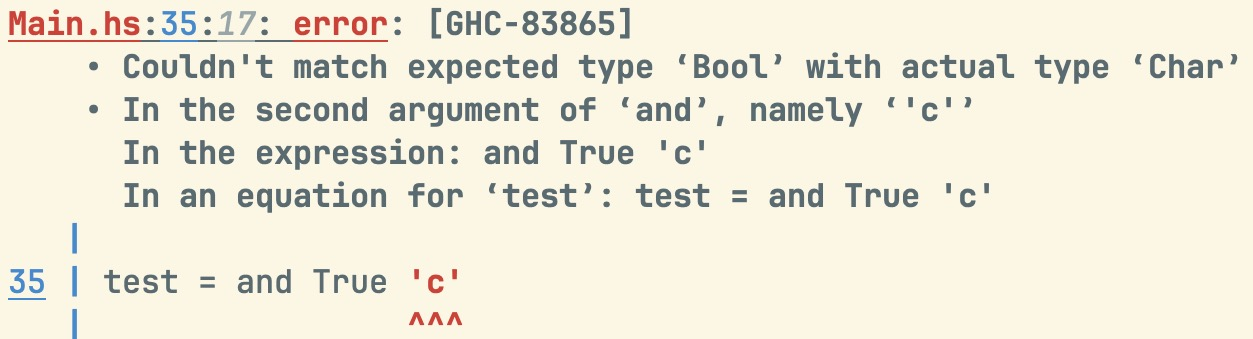
\includegraphics[width=\linewidth]{and-type-error}
  \end{figure}
\end{frame}

\section{Pure and Lazy Functional Programming}
\label{sec:pure-lazy-fp}

\begin{frame}[fragile]{Example: factorial in Python}
  \begin{figure}[H]
    \centering
    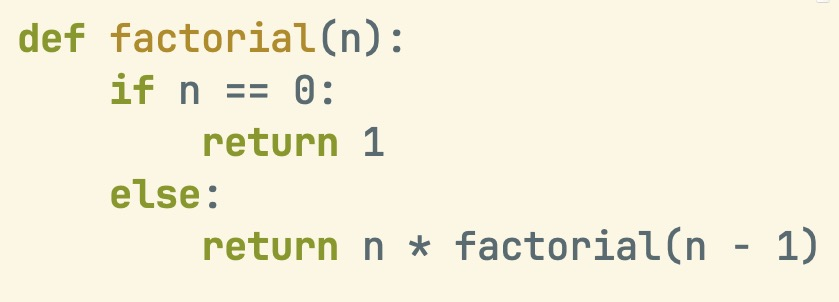
\includegraphics[width=\linewidth]{factorial-py}
  \end{figure}
\end{frame}

\begin{frame}[fragile]{Example: factorial in Haskell}
    \begin{figure}[H]
    \centering
    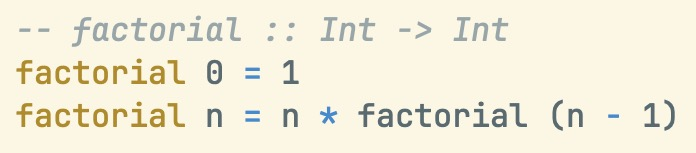
\includegraphics[width=\linewidth]{factorial-hs}
  \end{figure}

  \pause
  Let's evaluate \verb|factorial 3|:

  \begin{enumerate}
    \item<1-> \verb|factorial 3|
    \item<2-> \verb|3 * factorial 2|
    \item<3-> \verb|3 * 2 * factorial 1|
    \item<4-> \verb|3 * 2 * 1 * factorial 0|
    \item<5-> \verb|3 * 2 * 1 * 1|
    \item<6-> \verb|6 * 1 * 1|
    \item<7-> \verb|6 * 1|
    \item<8-> \verb|6|
  \end{enumerate}

\end{frame}

\begin{frame}[fragile]{Example: say in Python}

  \verb|say| is a function that given a number \textit{n} and a string \textit{string}, will repeat the \textit{string} \textit{n} times.

  e.g. \verb|say(2,"Hi ") = "Hi Hi "|

  \begin{figure}[H]
    \centering
    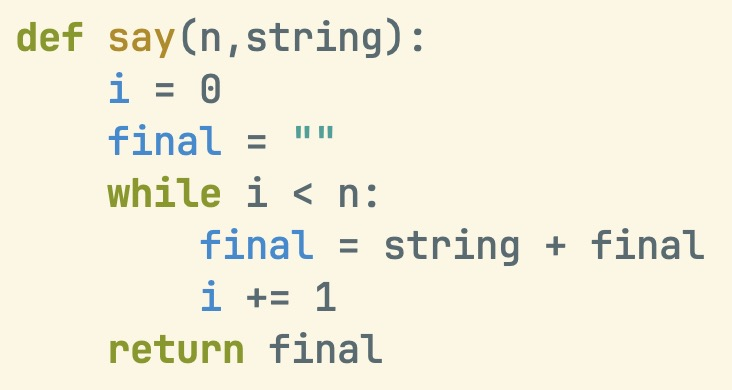
\includegraphics[width=\linewidth]{say-py}
  \end{figure}

\end{frame}

\begin{frame}[fragile]{Example: say in Haskell}
  The \verb|++| operator concatenates two strings together.

  \begin{figure}[H]
    \centering
    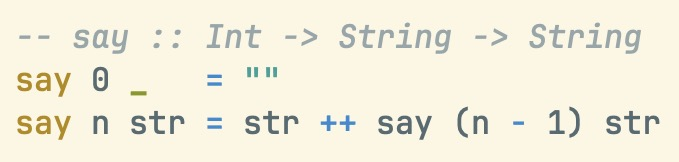
\includegraphics[width=\linewidth]{say-hs}
  \end{figure}

  \pause
  Let's evaluate \verb|say 2 "Hi "|:

  \begin{enumerate}
    \item<1-> \verb|say 2 "Hi "|
    \item<2-> \verb|"Hi " ++ say 1 "Hi"|
    \item<3-> \verb|"Hi " ++ "Hi " ++ say 0 "Hi"|
    \item<4-> \verb|"Hi " ++ "Hi " ++ ""|
    \item<5-> \verb|"Hi Hi " ++ ""|
    \item<6-> \verb|"Hi Hi "|
  \end{enumerate}

\end{frame}

\begin{frame}[fragile]{Example: hasEven in Python}
  \verb|hasEven| is a function that given a character, \textit{char}, and a string \textit{string}, will return \textit{true} if the number of times \textit{char} occurs in \textit{string} is even.

  \begin{figure}[H]
    \centering
    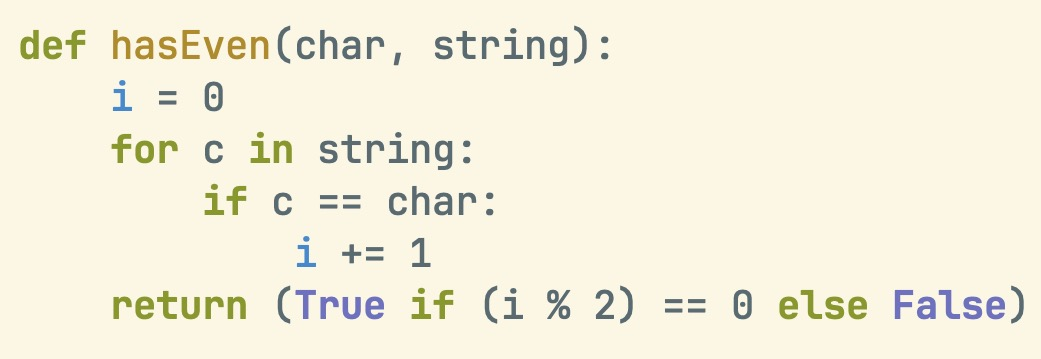
\includegraphics[width=\linewidth]{hasEven-py}
  \end{figure}

\end{frame}

\begin{frame}[fragile]{Example: hasEven in Haskell}
  \verb|even| is a built-in function that says whether its input is even or not.

    \begin{figure}[H]
    \centering
    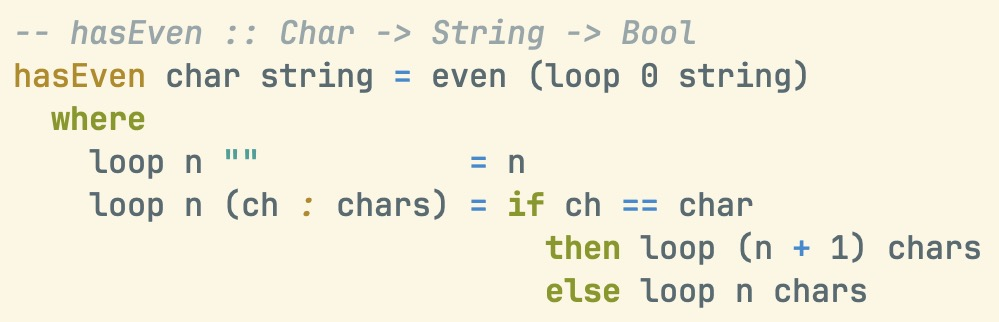
\includegraphics[width=\linewidth]{hasEven-hs}
  \end{figure}

  \pause
  Let's evaluate \verb|hasEven 'e' "eyes"|:

  \begin{enumerate}
    \item<1-> \verb|even (loop 0 "eyes")|
    \item<2-> \verb|even (loop 1 "yes")|
    \item<3-> \verb|even (loop 1 "es")|
    \item<4-> \verb|even (loop 2 "s")|
    \item<5-> \verb|even (loop 2 "")|
    \item<6-> \verb|even 2|
    \item<7-> \verb|True|
  \end{enumerate}

\end{frame}

\section{Influence of functional languages on imperative languages}
\label{sec:influence}

\section{Learning more}
\label{sec:learning-more}

\end{document}
